\documentclass{standalone}
\usepackage{tikz}
\usetikzlibrary{patterns, positioning}
\usetikzlibrary{shapes.misc}
\usepackage[outline]{contour}
\contourlength{1.5pt} 
\usepackage[sfdefault]{ClearSans} %% option 'sfdefault' activates Clear Sans as the default text font
\usepackage[T1]{fontenc}

\begin{document}
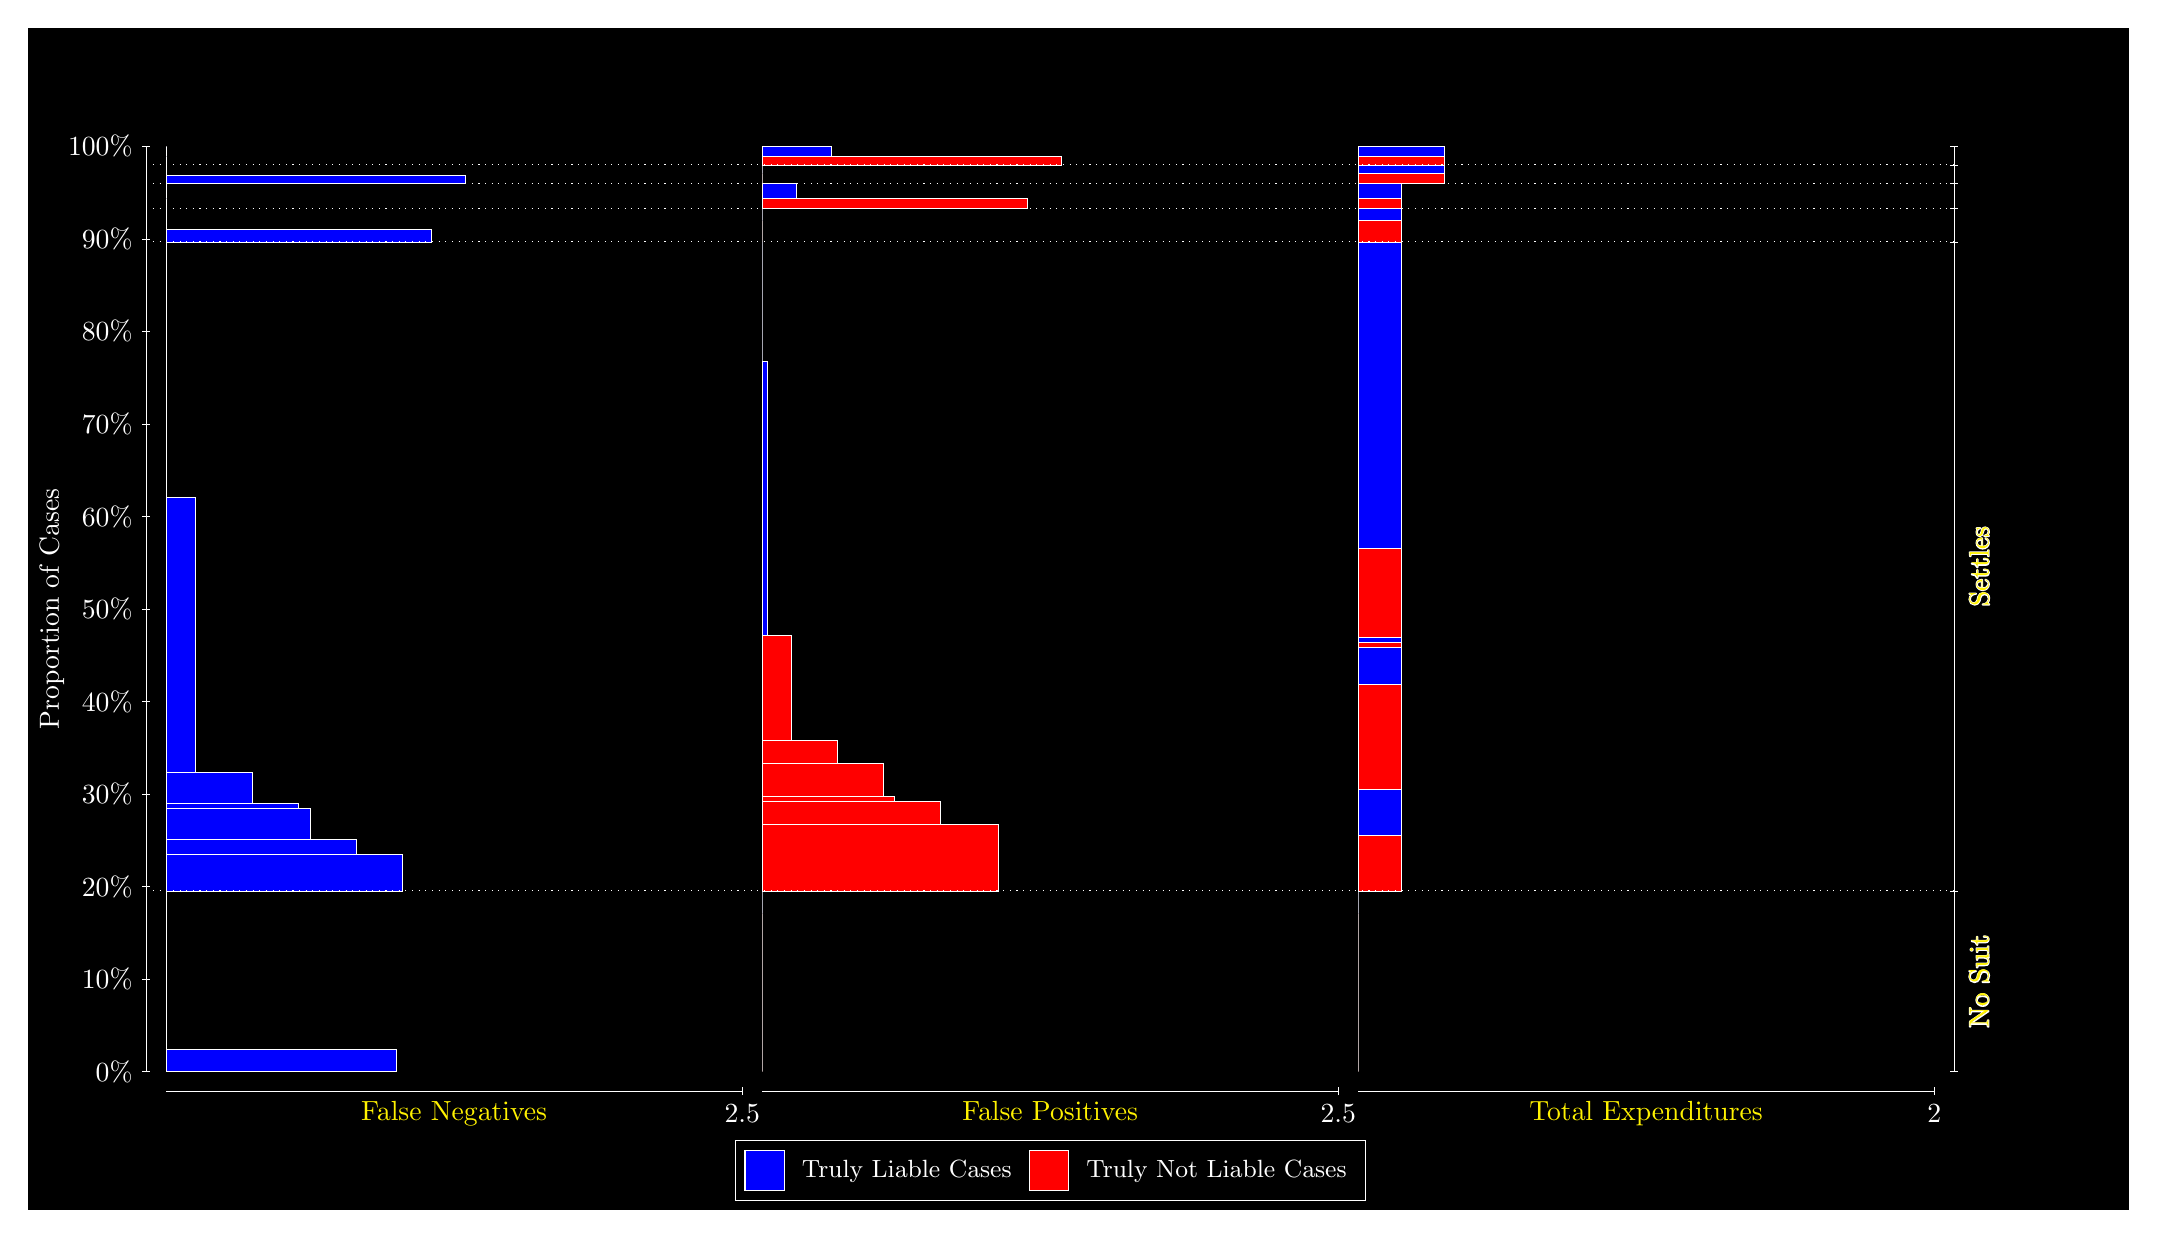
\begin{tikzpicture}
\draw[fill=black] (0,0) rectangle (26.667,15);
\draw[white, very thin] (1.5,1.75) -- (1.5,13.5);
\node[rotate=90, text=white, anchor=center] at (0.3, 7.625) {Proportion of Cases};
\draw[white, very thin] (1.45,1.75) -- (1.55,1.75);
\node[text=white, anchor=east] at (1.45, 1.75) {0\%};
\draw[white, very thin] (1.45,2.925) -- (1.55,2.925);
\node[text=white, anchor=east] at (1.45, 2.925) {10\%};
\draw[white, very thin] (1.45,4.1) -- (1.55,4.1);
\node[text=white, anchor=east] at (1.45, 4.1) {20\%};
\draw[white, very thin] (1.45,5.275) -- (1.55,5.275);
\node[text=white, anchor=east] at (1.45, 5.275) {30\%};
\draw[white, very thin] (1.45,6.45) -- (1.55,6.45);
\node[text=white, anchor=east] at (1.45, 6.45) {40\%};
\draw[white, very thin] (1.45,7.625) -- (1.55,7.625);
\node[text=white, anchor=east] at (1.45, 7.625) {50\%};
\draw[white, very thin] (1.45,8.8) -- (1.55,8.8);
\node[text=white, anchor=east] at (1.45, 8.8) {60\%};
\draw[white, very thin] (1.45,9.975) -- (1.55,9.975);
\node[text=white, anchor=east] at (1.45, 9.975) {70\%};
\draw[white, very thin] (1.45,11.15) -- (1.55,11.15);
\node[text=white, anchor=east] at (1.45, 11.15) {80\%};
\draw[white, very thin] (1.45,12.325) -- (1.55,12.325);
\node[text=white, anchor=east] at (1.45, 12.325) {90\%};
\draw[white, very thin] (1.45,13.5) -- (1.55,13.5);
\node[text=white, anchor=east] at (1.45, 13.5) {100\%};

\draw[white, very thin] (24.457,1.75) -- (24.457,13.5);
\draw[white, very thin] (24.407,1.75) -- (24.507,1.75);
\node[anchor=west] at (24.407, 1.75) {};
\draw[white, very thin] (24.407,4.0445) -- (24.507,4.0445);
\node[anchor=west] at (24.407, 4.0445) {};
\draw[white, very thin] (24.407,12.287) -- (24.507,12.287);
\node[anchor=west] at (24.407, 12.287) {};
\draw[white, very thin] (24.407,12.716) -- (24.507,12.716);
\node[anchor=west] at (24.407, 12.716) {};
\draw[white, very thin] (24.407,13.027) -- (24.507,13.027);
\node[anchor=west] at (24.407, 13.027) {};
\draw[white, very thin] (24.407,13.264) -- (24.507,13.264);
\node[anchor=west] at (24.407, 13.264) {};
\draw[white, very thin] (24.407,13.5) -- (24.507,13.5);
\node[anchor=west] at (24.407, 13.5) {};

\draw[white, very thin, fill=blue] (1.75,1.75) rectangle (4.6775,2.0365);
\draw[white, very thin, fill=red] (1.75,2.0365) rectangle (1.75,4.0445);
\draw[white, very thin, fill=blue] (1.75,4.0445) rectangle (4.7507,4.5088);
\draw[white, very thin, fill=blue] (1.75,4.5088) rectangle (4.1652,4.6992);
\draw[white, very thin, fill=blue] (1.75,4.6992) rectangle (3.5797,5.0959);
\draw[white, very thin, fill=blue] (1.75,5.0959) rectangle (3.4333,5.1533);
\draw[white, very thin, fill=blue] (1.75,5.1533) rectangle (2.8478,5.556);
\draw[white, very thin, fill=blue] (1.75,5.556) rectangle (2.1159,9.0455);
\draw[white, very thin, fill=red] (1.75,9.0455) rectangle (1.75,12.287);
\draw[white, very thin, fill=blue] (1.75,12.287) rectangle (5.1167,12.447);
\draw[white, very thin, fill=red] (1.75,12.447) rectangle (1.75,12.716);
\draw[white, very thin, fill=red] (1.75,12.716) rectangle (1.75,12.836);
\draw[white, very thin, fill=blue] (1.75,12.836) rectangle (1.75,13.027);
\draw[white, very thin, fill=blue] (1.75,13.027) rectangle (5.5558,13.133);
\draw[white, very thin, fill=red] (1.75,13.133) rectangle (1.75,13.264);
\draw[white, very thin, fill=red] (1.75,13.264) rectangle (1.75,13.369);
\draw[white, very thin, fill=blue] (1.75,13.369) rectangle (1.75,13.5);
\draw[white, very thin, fill=red] (9.3189,1.75) rectangle (9.3189,3.758);
\draw[white, very thin, fill=blue] (9.3189,3.758) rectangle (9.3189,4.0445);
\draw[white, very thin, fill=red] (9.3189,4.0445) rectangle (12.32,4.8927);
\draw[white, very thin, fill=red] (9.3189,4.8927) rectangle (11.588,5.18);
\draw[white, very thin, fill=red] (9.3189,5.18) rectangle (11.002,5.2451);
\draw[white, very thin, fill=red] (9.3189,5.2451) rectangle (10.856,5.659);
\draw[white, very thin, fill=red] (9.3189,5.659) rectangle (10.27,5.9511);
\draw[white, very thin, fill=red] (9.3189,5.9511) rectangle (9.6848,7.2861);
\draw[white, very thin, fill=blue] (9.3189,7.2861) rectangle (9.3921,10.776);
\draw[white, very thin, fill=blue] (9.3189,10.776) rectangle (9.3189,12.287);
\draw[white, very thin, fill=red] (9.3189,12.287) rectangle (9.3189,12.557);
\draw[white, very thin, fill=blue] (9.3189,12.557) rectangle (9.3189,12.716);
\draw[white, very thin, fill=red] (9.3189,12.716) rectangle (12.686,12.836);
\draw[white, very thin, fill=blue] (9.3189,12.836) rectangle (9.758,13.027);
\draw[white, very thin, fill=red] (9.3189,13.027) rectangle (9.3189,13.158);
\draw[white, very thin, fill=blue] (9.3189,13.158) rectangle (9.3189,13.264);
\draw[white, very thin, fill=red] (9.3189,13.264) rectangle (13.125,13.369);
\draw[white, very thin, fill=blue] (9.3189,13.369) rectangle (10.197,13.5);
\draw[white, very thin, fill=red] (16.888,1.75) rectangle (16.888,3.758);
\draw[white, very thin, fill=blue] (16.888,3.758) rectangle (16.888,4.0445);
\draw[white, very thin, fill=red] (16.888,4.0445) rectangle (17.437,4.7505);
\draw[white, very thin, fill=blue] (16.888,4.7505) rectangle (17.437,5.3376);
\draw[white, very thin, fill=red] (16.888,5.3376) rectangle (17.437,6.6726);
\draw[white, very thin, fill=blue] (16.888,6.6726) rectangle (17.437,7.1369);
\draw[white, very thin, fill=red] (16.888,7.1369) rectangle (17.437,7.202);
\draw[white, very thin, fill=blue] (16.888,7.202) rectangle (17.437,7.2593);
\draw[white, very thin, fill=red] (16.888,7.2593) rectangle (17.437,8.3948);
\draw[white, very thin, fill=blue] (16.888,8.3948) rectangle (17.437,12.287);
\draw[white, very thin, fill=red] (16.888,12.287) rectangle (17.437,12.557);
\draw[white, very thin, fill=blue] (16.888,12.557) rectangle (17.437,12.716);
\draw[white, very thin, fill=red] (16.888,12.716) rectangle (17.437,12.836);
\draw[white, very thin, fill=blue] (16.888,12.836) rectangle (17.437,13.027);
\draw[white, very thin, fill=red] (16.888,13.027) rectangle (17.986,13.158);
\draw[white, very thin, fill=blue] (16.888,13.158) rectangle (17.986,13.264);
\draw[white, very thin, fill=red] (16.888,13.264) rectangle (17.986,13.369);
\draw[white, very thin, fill=blue] (16.888,13.369) rectangle (17.986,13.5);
\draw[white, dotted] (1.5,4.0445) -- (24.457,4.0445);
\draw[white, dotted] (1.5,12.287) -- (24.457,12.287);
\draw[white, dotted] (1.5,12.716) -- (24.457,12.716);
\draw[white, dotted] (1.5,13.027) -- (24.457,13.027);
\draw[white, dotted] (1.5,13.264) -- (24.457,13.264);
\draw[white, very thin] (1.75,1.5) -- (9.0689,1.5);
\node[text=yellow, anchor=north] at (5.4094, 1.5) {False Negatives};
\draw[white, very thin] (9.0689,1.45) -- (9.0689,1.55);
\node[text=white, anchor=north] at (9.0689, 1.45) {2.5};

\draw[white, very thin] (9.3189,1.5) -- (16.638,1.5);
\node[text=yellow, anchor=north] at (12.978, 1.5) {False Positives};
\draw[white, very thin] (16.638,1.45) -- (16.638,1.55);
\node[text=white, anchor=north] at (16.638, 1.45) {2.5};

\draw[white, very thin] (16.888,1.5) -- (24.207,1.5);
\node[text=yellow, anchor=north] at (20.547, 1.5) {Total Expenditures};
\draw[white, very thin] (24.207,1.45) -- (24.207,1.55);
\node[text=white, anchor=north] at (24.207, 1.45) {2};

\node[text=yellow, centered, rotate=90] at (24.777, 2.8973) {\contour{white}{No Suit}};
\node[text=yellow, centered, rotate=90] at (24.777, 8.1658) {\contour{white}{Settles}};





\draw (12.978300999999998,1.5) node[draw=none] (baseCoordinate) {};
\begin{scope}[align=center]
        \matrix[scale=0.5, draw=white, below=0.5cm of baseCoordinate, nodes={draw}, column sep=0.1cm]{
            \node[rectangle, draw, minimum width=0.5cm, minimum height=0.5cm, fill=blue] {}; &
            \node[draw=none, font=\small, text=white] (B) {Truly Liable Cases}; &
            \node[rectangle, draw, minimum width=0.5cm, minimum height=0.5cm, fill=red] {}; &
            \node[draw=none, font=\small, text=white] (B) {Truly Not Liable Cases}; \\
            };
\end{scope}

\end{tikzpicture}
\end{document}